\documentclass[11pt]{article}

\usepackage[utf8]{inputenc}
\usepackage[T1]{fontenc}
\usepackage{ngerman, tikz}
\usetikzlibrary{calc, positioning}
\title{Versionsverwaltung von \LaTeX{}}
\author{Arne Brück}
\date{27.08.21}

\begin{document}
\maketitle

\section{Zusammenfassung}
Wer von Git höhrt, denkt häufig an GitHub, den Ort, der die Hälfte der
Software der Welt enthält und von dem sich die ganze Welt die Software
frei herunterladen kann.

Git ist aber unabhängig von GitHub, es ist ein Programm zur
Versionsverwaltung. Es ermöglicht auf einfache Weise Sicherheitskopien
des Projektes zu erstellen und zu späteren Zeitpunkten auf alle
früheren Veränderungen zugreifen zu können. Dies soll anhand dieses
Projektes verdeutlicht werden. Zusätzlich kann im Anschluss über
GitHub das Projekt gesichert werden oder mit anderen Menschen zusammen
komfortabel an diesem gearbeitet werden.

\section{Grundlagen}

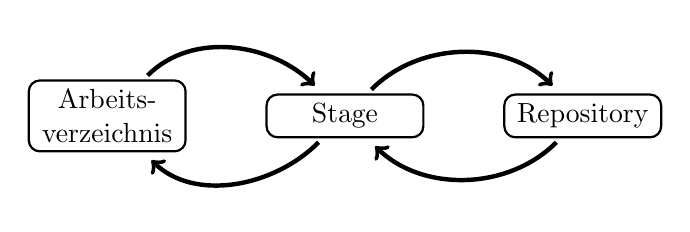
\begin{tikzpicture}
  \node (AV) [thick, draw, rounded corners, rectangle, text width = 5em, text
  centered] {Arbeits\-verzeichnis};
  \node (Stage) [thick, draw, rounded corners, rectangle, text width = 5em, text
  centered, right = of AV ] {Stage};
  \node (Rep) [thick, draw, rounded corners, rectangle, text width = 5em, text
  centered, right  = of Stage] {Repository};
  \draw [ultra thick, ->, shorten >=4pt, shorten <=2pt] (AV) to [out = 45, in = 135] (Stage);
  \draw [ultra thick, ->, shorten >=4pt, shorten <=2pt] (Stage) to [out = 225, in = -45]  (AV);
  \draw [ultra thick, ->, shorten >=4pt, shorten <=2pt] (Stage) to [out = 45, in = 135] (Rep);
  \draw [ultra thick, ->, shorten >=4pt, shorten <=2pt] (Rep) to [out = 225, in = -45]  (Stage);
\end{tikzpicture}

Das \textbf{Arbeitsverzeichnis} ist das normaler Verzeichnis, in dem auf dem
Computer die Dateien gespeichert werden.

Das \textbf{Repository} (Repo) ist der Inhalt des Arbeitsverzeichnis in allen
gespeicherten Varianten. Wurde im Arbeitsverzeichnis beispielsweise
eine Datei irrtümlicherweise gelöscht, kann ein älterer Stand des
Arbeitsverzeichnisses wiederhergestellt werden, um die Datei
wiederzubekommen. Hierfür muss natürlich vorher der Inhalt des
Arbeitsverzeichnisses im Repo gespeichert werden. Dies erfolgt
gewöhnlich immer, wenn eine Sinneinheit abgeschlossen worden ist. Hier
zum Beispiel vor und nach Erstellen des Diagramms. Das Speichern im
Repo wird als \textsl{Commit} bezeichnet.

Die \textbf{Stage} steht zwischen Arbeitsverzeichnis und Repository.
Ein Commit ist immer ein wesentlicher Schritt, der genau dokumentiert
wird und für alle anderen Menschen auf Ewigkeit sichtbar ist. Daher
werden alle Änderungen zuerst auf die Stage (Bühne) gesetzt und vor
dem Commit gründlich geprüft. Idealerweise sollte das folgende Commit
nicht 1 Minute später mit dem Kommentar \textsl{Diese Datei hatte ich
  vergessen} erfolgen.

\end{document}

%%% Local Variables:
%%% mode: latex
%%% TeX-master: t
%%% End:
